
% the LaTeX macro package from Springer-Verlag
% for Lecture Notes in Computer Science,
% version 2.4 for LaTeX2e as of 16. April 2010


%\bibliographystyle{splncs}


\documentclass[runningheads,a4paper]{llncs}
%\usepackage{natbib}
%\usepackage{cite}
\usepackage{amssymb}
\setcounter{tocdepth}{3}
\usepackage{graphicx}

\usepackage{url}

\usepackage{listings}

\usepackage{color}

\definecolor{darkgreen}{rgb}{0.0, 0.2, 0.13}
\definecolor{dkgreen}{rgb}{0,0.6,0}
\definecolor{gray}{rgb}{0.5,0.5,0.5}
\definecolor{mauve}{rgb}{0.58,0,0.82}
\definecolor{lightgray}{rgb}{0.83, 0.83, 0.83}
\definecolor{platinum}{rgb}{0.9, 0.89, 0.89}
\definecolor{magnolia}{rgb}{0.97, 0.96, 1.0}
\definecolor{floralwhite}{rgb}{1.0, 0.98, 0.94}



\lstdefinestyle{customtext}{
backgroundcolor=\color{floralwhite},
 basicstyle=\fontsize{8}{10}\ttfamily,
  columns=fullflexible,
  breaklines=true%,
  %postbreak=\raisebox{0ex}[0ex][0ex]{\color{mauve}$\hookrightarrow$\space}
}


\lstdefinestyle{customcode}{
backgroundcolor=\color{platinum},
language=Python,
showstringspaces=false,
columns=flexible,
basicstyle={\small\ttfamily},
keywordstyle=\color{blue},
stringstyle=\color{mauve},
commentstyle=\color{mauve}\ttfamily
}



\usepackage{hyperref}

\begin{document}

\pagestyle{headings}  % switches on printing of running heads
\addtocmark{Bloatectomy} % additional mark in the TOC

%
%\tableofcontents
%
\mainmatter              % start of the contributions

\title{Bloatectomy:}
\subtitle{A method for the identification and removal of duplicate text in the bloated notes of electronic health records and other documents}

\titlerunning{Bloatectomy}  % abbreviated title (for running head)

\author{Summer K Rankin$^{*}$\inst{1}  \and Roselie Bright\inst{2} \and Katherine Dowdy\inst{1}}

\authorrunning{Rankin, Bright \& Dowdy, 2020} % abbreviated author list (for running head)

\institute{Booz Allen Hamilton, McLean, VA, USA\\
%orcid: 0000-0002-6886-3983\\
\email{rankin\_summer@bah.com}\\
\and
Office of Health Informatics, Office of the Chief Scientist, Office of the Commissioner, \\U.S. Food and Drug Administration,
Rockville, MD, USA, \\%orcid: 0000-0002-7565-1284\\
\email{roselie.bright@fda.hhs.gov}\\  
$*$Corresponding Author\\
The authors are listed in order of contributions to the work and manuscript.}

\maketitle              % typeset the title of the contribution

\begin{abstract}
Duplicated sentences (“note bloat”) in unstructured electronic healthcare records hamper scientific research. Existing methods did not meet our needs. We adapted the LZW compression algorithm into a new method and designed parameters to allow customization for varying data and research needs. This resulted in the Bloatectomy package which identifies duplicate sentences in unstructured healthcare notes (or other documents), marks them for manual review, and removes them for statistical analysis. The package allows for a high level of customization in the length and type of duplications (via regular expressions) and could also be used for plagiarism detection or other text pre-processing requirements for natural language processing (NLP). The Bloatectomy package works, is available for use, and can be adapted for other settings. Bloat-ectomy is free, open source, and released under the GNU General Public License v3.0.

\textbf{url:} \url{https://github.com/MIT-LCP/bloatectomy}\\  
\textbf{pypi:} \url{https://pypi.org/project/bloatectomy/}\\  
\textbf{anaconda:} \url{https://anaconda.org/summerkrankin/bloatectomy}  

\keywords{ python, medical informatics, electronic health records,  electronic medical records,  public health informatics, clinical information extraction, health informatics, natural language processing, data augmentation}
\end{abstract}



\section{Introduction}

\noindent The authors are part of a team that is using the text notes in electronic healthcare records (EHRs). Our EHRs are a de-identified hospital critical care data set known as the Medical Information Mart for Intensive Care (MIMIC-III) \cite{mimiciii} \cite{mimiciiidata} \cite{physionet}.


\begin{figure}
\center{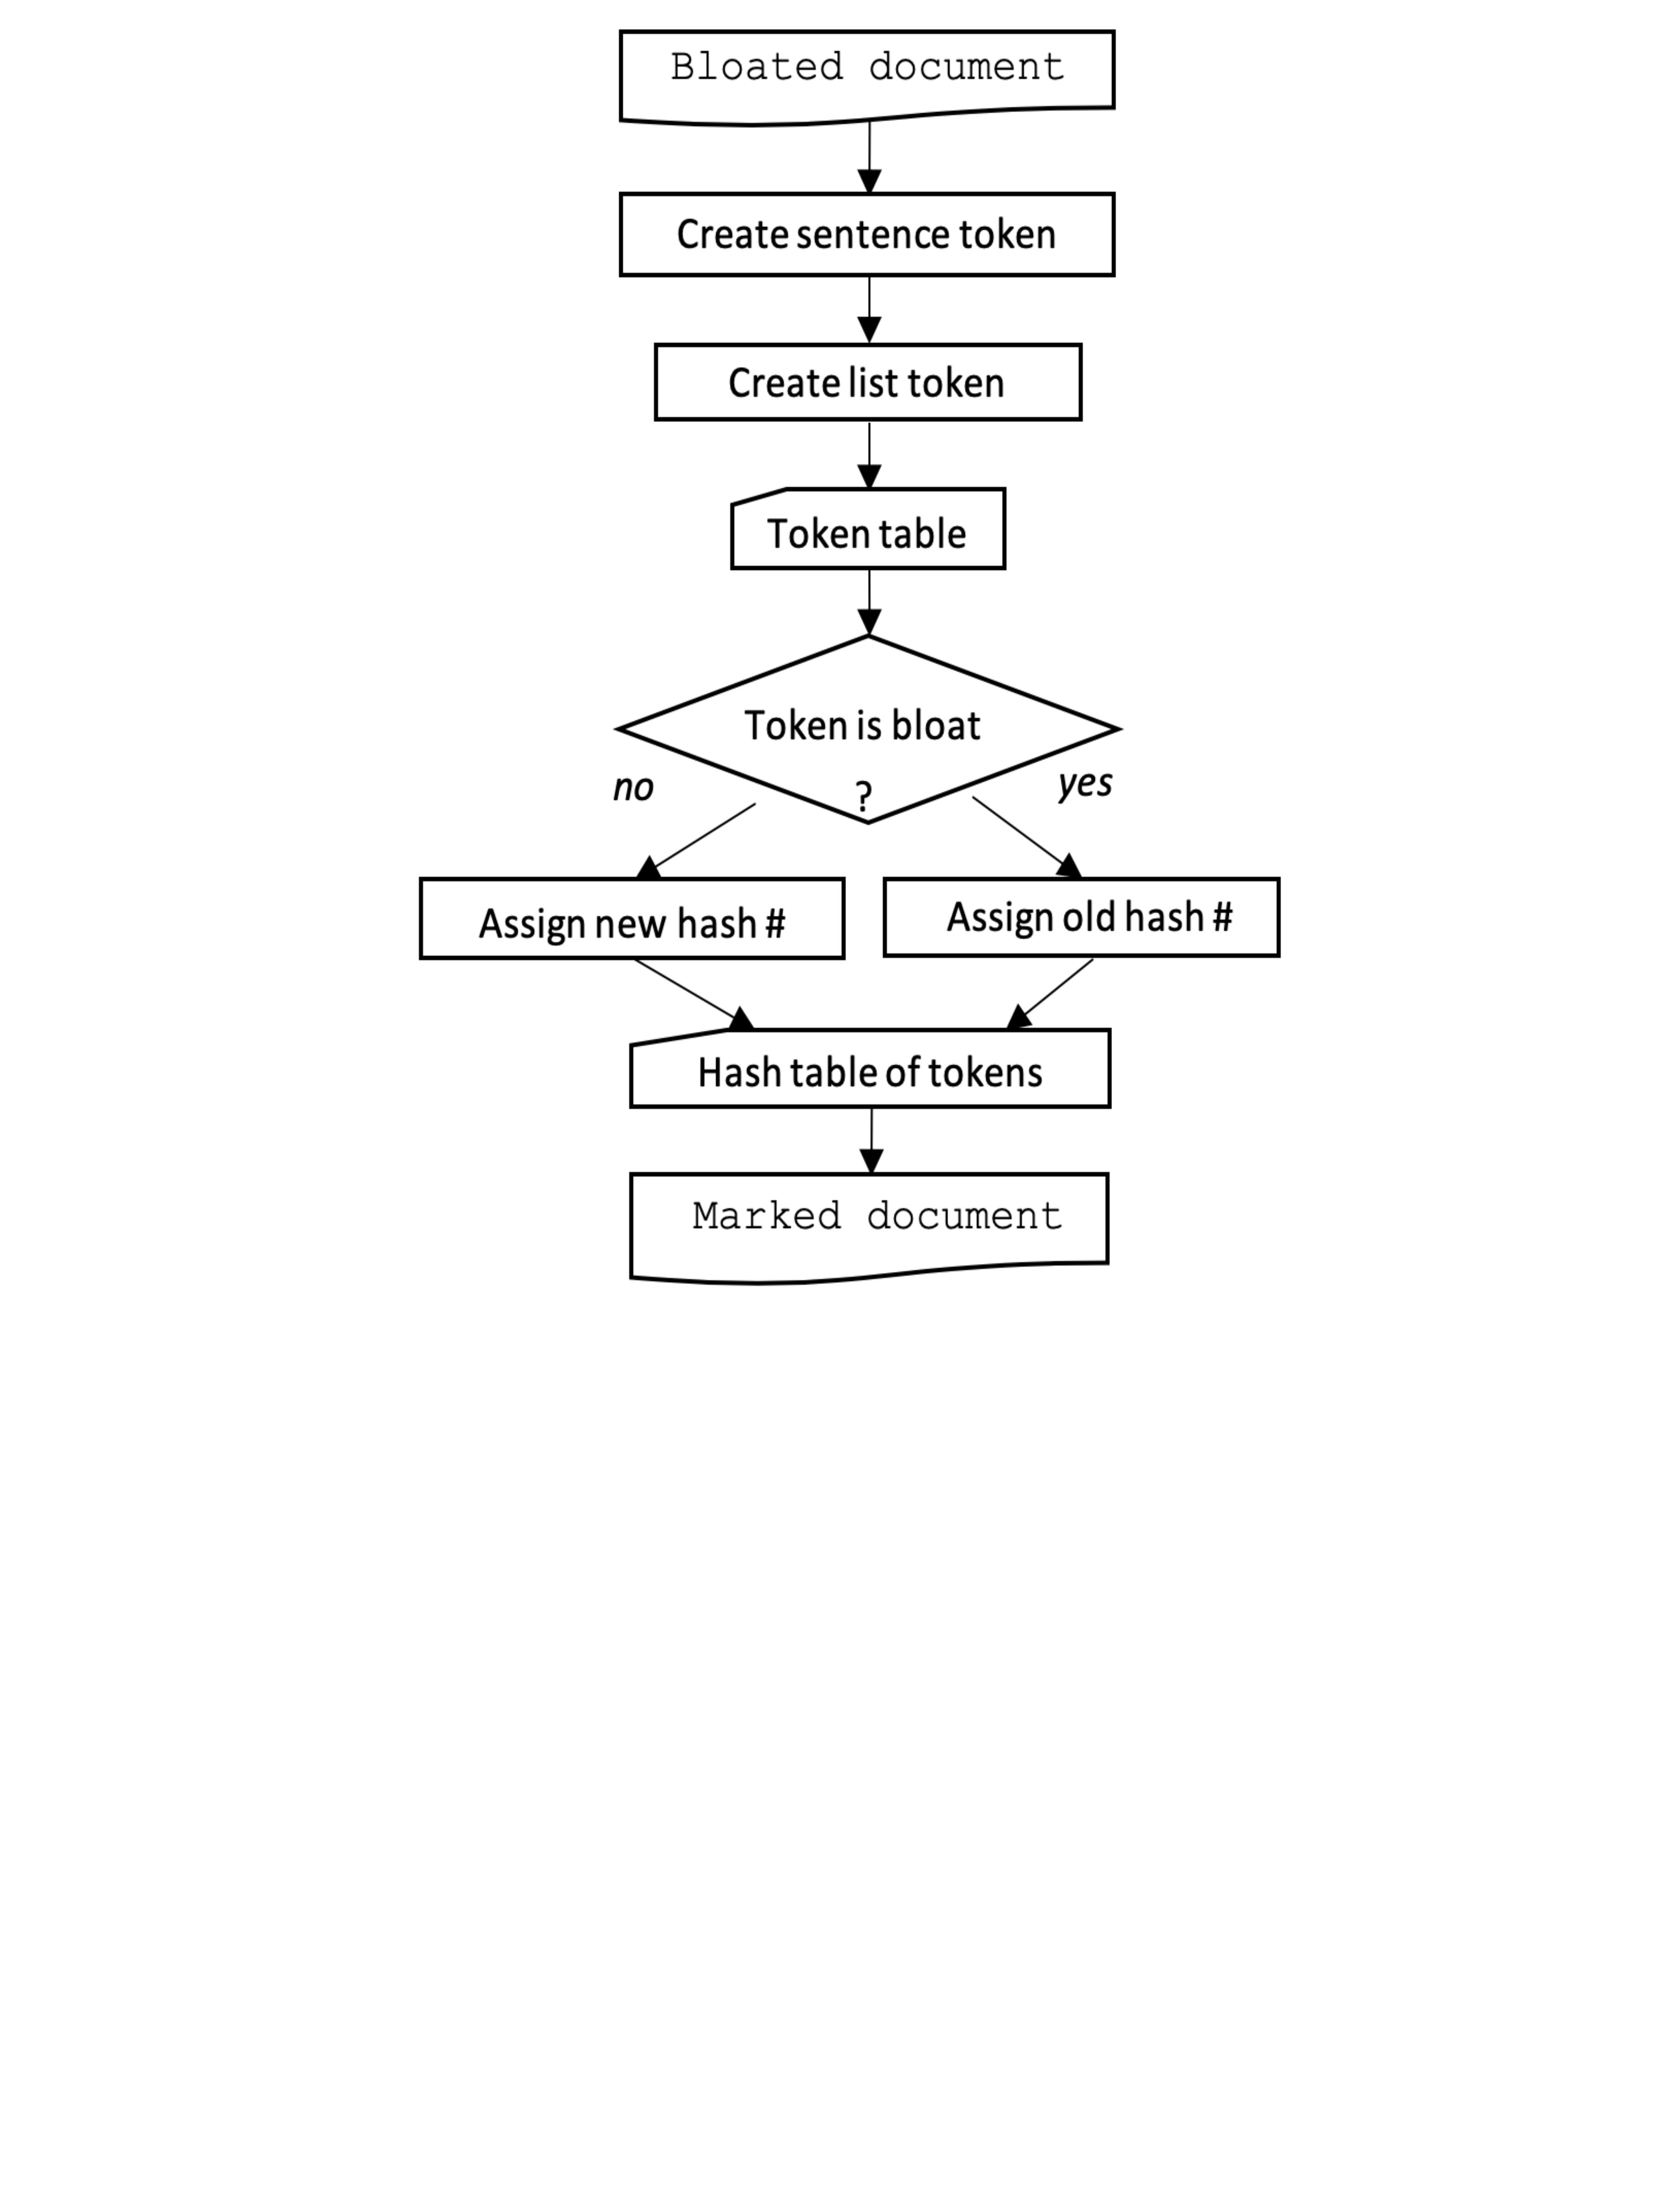
\includegraphics[height=2.25in]{graph_abstract.png}}
 \caption {\textbf{Graphical Abstract}}
 \label{abstract}
\end{figure}


\noindent Most notes were made by physicians (attending, radiology, consulting) and CCU nurses. Most of these notes included sections that were duplicates of earlier notes (written by themselves or another provider) for the same patient’s hospitalization (their admission). Sometimes pasted sections were edited, and then the modified text was duplicated into later notes (see Figures \ref{notes1} and \ref{notes2}).

\begin{figure}
\center{\includegraphics[height=.70in]{notes1.png}}
 \caption {\textbf{Progressively longer nurse’s notes over one shift.} In this figure, we used a manual method to highlight identical sentences with unique colors. The original sentences are in bold font as well. This and similar figures in this document are purposely small and low resolution to provide further patient and provider privacy protection without disturbing our point about duplicate text.}
 \label{notes1}
\end{figure}

\begin{figure}
\center{\includegraphics[height=1.1in]{notes2.png}}
 \caption {\textbf{ Example of two physicians’ notes from the same time period.} In this figure, we used a manual method to highlight identical sentences with unique colors. The original sentences are in bold font as well.}
 \label{notes2}
\end{figure}

\noindent This type of duplication has been noticed in other health care settings (reviewed in \cite{Dean:2018}). The duplications distort statistical analyses of terms used and hamper manual review of the notes for changes in patient care and status. Removing these duplicated notes allows us to use a wide variety of statistical methods without concern for the weights introduced by duplicates. \\
\\

\noindent For example, if we are using a simple frequency (count) vectorization method, the more times a word appears, the more important it is in the analysis. Furthermore, as length of stay increases, the burden of duplicates also increases, which inflates the importance of, for example, admission comments. Artificial repeats (copies) of text will artificially inflate the importance of the repeated words or phrases \cite{Cohen:2013}. Though existing methods can weight words (i.e., term-frequency x inverse document frequency (TF-IDF)), for this dataset these methods did not yield satisfactory results.\\
\\

\noindent Our goal was to identify duplicated sections to aid manual review and to delete them from statistical processes. We developed criteria for the tool that were based on the clinical setting and our desire to keep all new clinical information. Specifically:


\begin{enumerate}
\item
Minimum clinical concepts were at the sentence or partial or complete list level.  Minor changes within a sentence or list could change the clinical meaning; for example, insertion of the word “not” reverses the meaning of a sentence. We wanted a tool that would find exact duplicate sentences and lists.
\medskip

\item
Duplications could occur as an entire note or partial note. We wanted to find both partial and entire duplicates of notes.
\medskip

\item
Duplications from more than one original source could occur in a single note, and we wanted to find all of them.
\medskip

\item
Exact or partial duplications could occur across many notes, and we wanted to find all of them.
\medskip

\item
Lists of clinical parameters and values could be completely or partially duplicated across notes. In addition to finding duplicates of entire lists, we wanted to find duplicates of significantly long sections of lists in the notes.
\medskip

\item
Document structure (headings, paragraph formats, list formats) of notes varied widely. We needed a method with broad independence of the internal structures.
\medskip

\item
We wanted the method to be simple and user-friendly if doing so resulted in an acceptably low level of error.
\medskip

\item
We wanted to be able to use the output for two purposes:
\begin{enumerate}
\item
Aid manual review of notes by marking the duplicate sections
\medskip

\item
Statistical analyses
\end{enumerate}
\end{enumerate}    

\medskip

\noindent We evaluated existing available tools and strategies:
\begin{itemize}
\item
Plagiarism tools typically compare documents and stop after finding the first instance of duplicate text \cite{Su:2008} \cite{copyfind} \cite{Ceglarek:2013}; some also appropriately account for paraphrasing. Some other duplication detection methods \cite{Thielke:2007} \cite{Wrenn:2010} rely on the Bloomfield plagiarism tool. We focused on concepts at the sentence level because word meaning depends on its immediate sentence and paragraph, regardless of where it appears in the note. Genetic and protein sequence comparators also finish after finding similar sequences \cite{Altschul:1990}. We wanted to find exact duplicates and every instance of them.
\medskip
\item
Some existing EHR deduplication methods have been applied only to the discharge note \cite{Cohen:2013}. Unfortunately, the discharge notes in MIMIC III are not comprehensive accounts of all observations and treatments that may be key to specific research questions; for example, blood transfusions are sometimes noted in coded data or nursing notes yet were absent from the discharge summary.
\medskip
\item
Fingerprinting identifies redundant entire notes based on similarity \cite{Cohen:2013}, but it finds inexact duplicates (which could be clinically different in some way). Also, we wanted to identify duplicate concepts within notes even if some other parts of the note were original.
\medskip

\item
Clustering entire notes, and then looking for entire and near duplicate pairs of notes within clusters \cite{Gabriel:2018} works only on entire notes. We wanted to detect duplicate sentences and lists within notes, even if new material existed among the duplicates.
\medskip

\item
Detecting duplicates through topic modeling, an unsupervised and unreplicable \cite{Lancichinetti:2015} method of clustering related words and expressions within documents, \cite{Cohen:2014} involved comparing two simplifications that did not fit our needs

\begin{itemize}
\medskip

\item
Selection and use of a best note within the admission. We found that crucial clinical information was missing from any one best note in an admission.
\medskip

\item
Selection of the one source note, the longest one, in the admission.  We found that in MIMIC III, there is no single source note in an admission.
\end{itemize}
\medskip

\item
Sliding windows (\cite{Zhang:2011}), similar to frameshifting in other fields, were a possibility if we adapted them to sentences and lists. We believe our method is simpler to implement.
\end{itemize}
\bigskip

\noindent The LZW compression algorithm \cite{Welch:1984} hashes words by assigning sequential numeric addresses to them. Any word that has been hashed before is assigned the original numeric address. We adapted the method to sentences rather than words because the altered sentences in pasted text also had new meanings. The hashing system allowed us to both highlight pasted sentences in text documents and remove the duplicate sentences during preprocessing for statistical analysis.

\section{Duplicate Detection}
\begin{figure}
\center{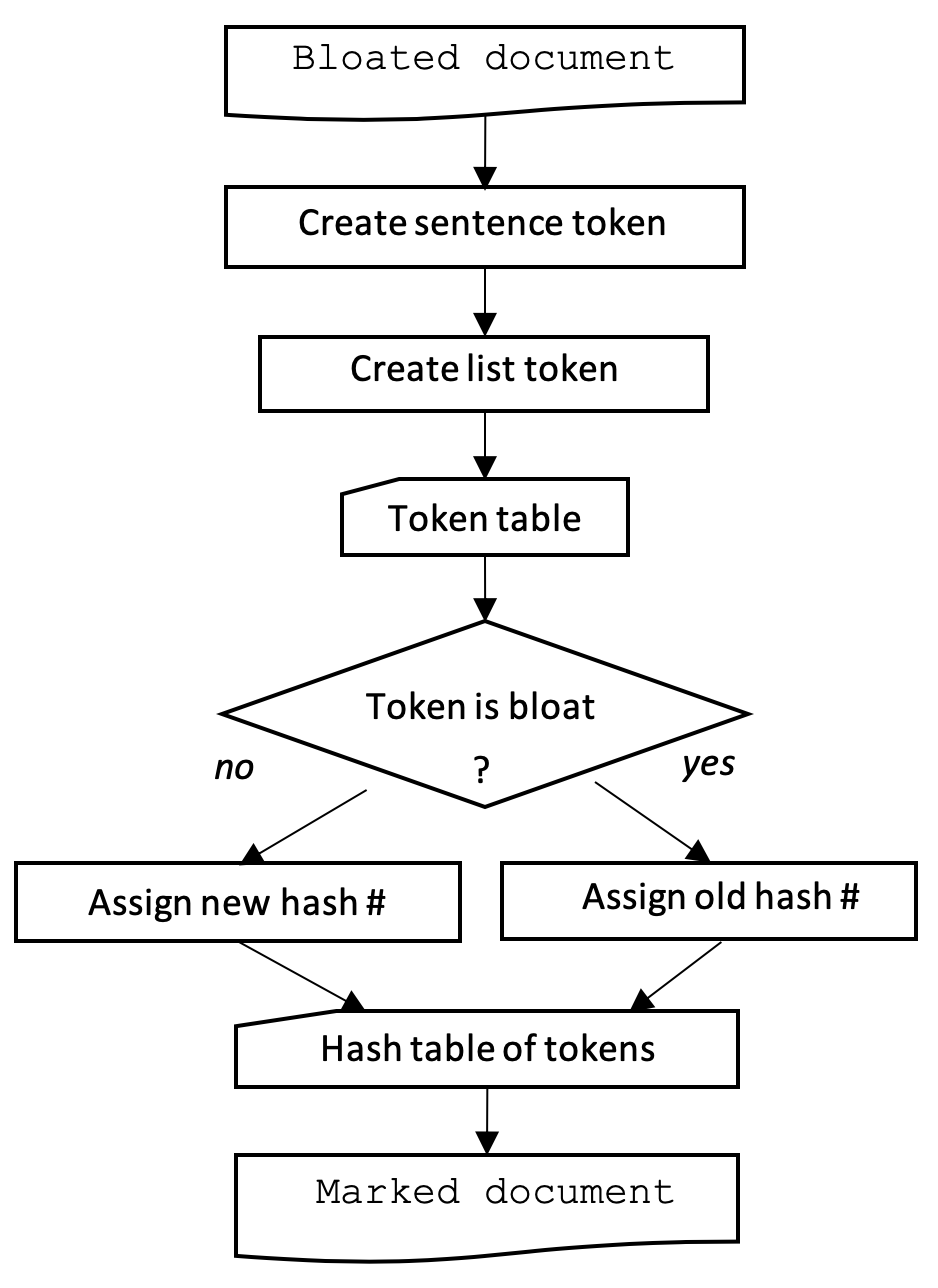
\includegraphics[height=3.0in]{flowchart.png}}
 \caption {\emph{High-level flowchart of the Bloatectomy method.}}
 \label{flowchart}
\end{figure}

\subsection{Document Selection}
\noindent In Natural Language Processing (NLP), we refer to a unit of text as a document. In the MIMIC-III database, free-text notes from multiple sources are associated with a patient's admission (HADM\_ID). For our analysis, a document consisted of the concatenation of all notes for an admission into one single document in chronological order. Thus, there is one document per admission.

\subsection{Code and Example}
\noindent The Bloatectomy (v.2.1) tool can be found in the python package \textbf{bloatectomy.py}. The MIMIC-III database was stored in a PostgreSQL (v.9.4) database. The Bloatectomy tool was written using only Python 3 (v.3.7.3) \cite{python3}. No other libraries are needed to identify duplicate text. An option to ingest or output a word document requires the python-docx library.


\noindent The Bloatectomy method is as follows:
\begin{enumerate}
\item
Create sentence tokens.
\item
Create list tokens.
\item
Assign either new or old hash number.
\item
Use the hash table of tokens to:
\begin{itemize}
\item
Mark duplicate tokens in a recreated document for manual review.
\item
Create a string from the unduplicated tokens for statistical analysis.
\end{itemize}
\end{enumerate}


\subsubsection{Create Sentence Tokens}
\noindent First, we tokenized (separated) an admission's concatenated notes (a single document) based on the presence of:
\begin{itemize}
\item
a period ($.$)followed by one or more
\item
white space characters (space, tab, line break) or 
\item
line feed character (\textbackslash{}n). 
\end{itemize}

\noindent An example of the text seen in an EHR looks like the following:


\begin{lstlisting}[frame=single, style=customtext]
No CP. Became tachycardic to 160s on dopa. No CP.
Tmax: 36.6
C (97.8
HR: 100 (97 - 166) bpm
Tmax: 36.6
C (97.8
\end{lstlisting}



\noindent The plain text--i.e., only the characters used to represent the text--looks like the following:


\begin{lstlisting}[frame=single, style=customtext]
No CP. Became tachycardic to 160s on dopa. No CP.\nTmax: 36.6\nC (97.8\nHR: 100 (97 - 166) bpm\nTmax: 36.6\nC (97.8
\end{lstlisting}

\noindent The first tokenization was accomplished using a regular expression \ref{regex1} in python (v.3.7.3) using the \textbf{re} (regular expression) library. This regular expression can be changed by passing any valid regular expression for the \verb|regex1=| parameter.

\begin{figure}
\center{\includegraphics[height=.75in]{regex1.png}}
 \caption {\emph{The regular expression used for the first tokenization.}}
 \label{regex1}
\end{figure}

\noindent At this point, we have two tokens because there are two periods followed by a line feed character  (\textbackslash{}n).

\medskip\noindent%{\itshape Sample Output}
\begin{table}
\caption{Tokens after first tokenization}
\begin{center}
\renewcommand{\arraystretch}{1.4}
\setlength\tabcolsep{3pt}
\begin{tabular}{lll}
\hline\noalign{\smallskip}
Token Number & Token\\
\noalign{\smallskip}
\hline
\noalign{\smallskip}
 1 & No CP.\\
 2 & Became tachycardic to 160s on dopa. \\
3 & No CP. \\
4 & \verb|\nTmax: 36.6\nC (97.8\nHR: 100 (97 - 166) bpm\nTmax: 36.6\nC (97.8| \\

\hline
\end{tabular}
\end{center}
\end{table}

\subsubsection{Create List Token}
\noindent Next, each token is examined and split again if it contains a line feed character followed by one or more:

\begin{itemize}
\item
Upper case character
\item
Digit
\item
En dash (-)
\item
Number sign (\#)  
\end{itemize}


\noindent Using our sample text, \textbf{token 4} is split into several new tokens, which are then inserted into our token list. If a token does not need to be split further, it is added to our list as-is. The regular expression for the split shown in \ref{regex2}. This regular expression can be changed by passing any valid regular expression for the \verb|regex2=| parameter.

\begin{figure}
\center{\includegraphics[height=.75in]{regex2.png}}
 \caption {\emph{The regular expression used to calculate the second tokenization.}}
 \label{regex2}
\end{figure}

\noindent After the token has been split, the text is cleaned up to increase the matches and focus on the text rather than the formatting. All line feed characters are replaced with one white space. White spaces at the beginning and end of a token are removed, then the token is added to the new token list.

\begin{lstlisting}[frame=single, style=customcode]

# replace \n with a space with a space
sent_token = [re.sub(r"$\n+","",i) for i in sent_token] # remove end
sent_token = [re.sub(r"^\n", "", i) for i in sent_token] #remove front

# line feeds + whitespace or not
sent_token = [re.sub(r"\s+\n\s+", " ", i) for i in sent_token]
sent_token = [re.sub(r"\s+\n", " ", i) for i in sent_token]
sent_token = [re.sub(r"\n\s+", " ", i) for i in sent_token]
sent_token = [re.sub(r"\n", " ", i) for i in sent_token]

#remove front/end whitespace
sent_token = [i.strip(' ') for i in sent_token]
\end{lstlisting}


\noindent Specifically, \textbf{token 4} becomes 5 new tokens:

\medskip\noindent%{\itshape Sample Output}
\begin{table}
\caption{Tokens after second tokenization}
\begin{center}
\renewcommand{\arraystretch}{1.4}
\setlength\tabcolsep{3pt}
\begin{tabular}{lll}
\hline\noalign{\smallskip}
Token Number & Token\\
\noalign{\smallskip}
\hline
\noalign{\smallskip}
 1 & No CP.\\
 2 & Became tachycardic to 160s on dopa. \\
3 & No CP. \\
4 & Tmax: 36.6 \\
5 & C (97.8 \\
6 & HR: 100 (97 - 166) bpm\\
7 & Tmax: 36.6 \\
8 & C (97.8\\
\hline
\end{tabular}
\end{center}
\end{table}

\subsubsection{Assign Either New or Old Hash Number}
Next, we create a dynamic set structure that accepts tokens one at a time. The function is a generator that yields one token at a time; when the output is stored as a list, the original order of tokens is maintained while providing the flexibility to either remove or mark (highlight, bold) a duplicate token.

\noindent As each token is passed through the loop, one of two outcomes will result:
\begin{enumerate}
\item
If the token is not in the dynamic set, it will be added to the set, and the token is yielded as-is.
\medskip

\item
If the token is already contained in the set, it is NOT added to the set; HTML tags are added to the token, yielding a marked token. If we want to remove the token, nothing is yielded at this step.
\end{enumerate}

\begin{lstlisting}[frame=single, style=customcode]
tokens_set = set()
tokens_set_add = tokens_set.add

for token in input_tokens:

  if token == '':
    pass

  elif token not in tokens_set:
    tokens_set_add(token)
    yield token

  elif remov == False:
    yield tag + token + tag_end

  elif remov == True:
    pass
\end{lstlisting}


\noindent The token table essentially becomes the following hash table of tokens:

\medskip\noindent%{\itshape Sample Output}
\begin{table}
\caption{Hash Table of Tokens}
\begin{center}
\renewcommand{\arraystretch}{1.4}
\setlength\tabcolsep{3pt}
\begin{tabular}{lllll}
\hline\noalign{\smallskip}
Token Number & Token & Is Bloat & Hash Number\\
\noalign{\smallskip}
\hline
\noalign{\smallskip}
 1 & No CP. & No & 1\\
 2 & Became tachycardic to 160s on dopa. & No &2 \\
duplicate & \verb|<mark>No CP.</mark> | &Yes &1\\
4 & Tmax: 36.6 & No & 3\\
5 & C (97.8 & No & 4\\
6 & HR: 100 (97 - 166) bpm & No & 5\\
duplicate & \verb|<mark>Tmax: 36.6</mark>| & Yes & 3\\
duplicate & \verb|<mark>C (97.8</mark>| & Yes & 4\\
\hline
\end{tabular}
\end{center}
\end{table}


\subsubsection{Use the Hash Table of Tokens}
\noindent The output is a document with a list of our original tokens with highlight formatting marks around the duplicates. The user can choose to highlight, bold, or remove duplicates by setting the verb|style=| argument.

\begin{lstlisting}[frame=single, style=customcode]
import bloatectomy from bloatectomy
bloatectomy(text, style='highlight'))
\end{lstlisting}

\medskip\noindent%{\itshape Sample Output}
\begin{table}
\caption{Marked Table of Tokens}
\begin{center}
\renewcommand{\arraystretch}{1.4}
\setlength\tabcolsep{3pt}
\begin{tabular}{llllll}
\hline\noalign{\smallskip}
Token Number & Token\\
\noalign{\smallskip}
\hline
\noalign{\smallskip}
 1 & No CP.\\
 2 & Became tachycardic to 160s on dopa. \\
duplicate & \verb|<mark>No CP.</mark> |\\
4 & Tmax: 36.6 \\
5 & C (97.8 \\
6 & HR: 100 (97 - 166) bpm\\
duplicate & \verb|<mark>Tmax: 36.6</mark>| \\
duplicate & \verb|<mark>C (97.8</mark>|\\
\hline
\end{tabular}
\end{center}
\end{table}


\noindent Last, we concatenate this marked (or de-duplicated) set of tokens together to create a document of original sentences. A line feed is placed between each token for ease of viewing (due to removing the line feed characters at the beginning and end of each token). How this is executed depends on the type of output (e.g., docx, HTML).

\begin{lstlisting}[frame=single, style=customcode]
uniq = str("\n".join(text))
\end{lstlisting}


\noindent The final output (\ref{output}) contains three highlighted duplicate tokens:  
\begin{figure}
\center{\includegraphics[height=1.0in]{example_output.png}}
 \caption {\emph{ Highlighted duplicates in the output from the example text.} }
 \label{output}
\end{figure}

\noindent The marked text can be deleted for statistical analyses.  

\begin{lstlisting}[frame=single, style=customcode]
bloatectomy(text, style='remov'))
\end{lstlisting}

\subsection{Parameter Adjustments}
\noindent We incorporated parameters that users can set to fit the features of the documents they are using. The following input types can be used:
\begin{enumerate}
\item
Plain text files (.txt, .rtf)
\item
Word documents (.docx)
\item
A variable containing a string of raw text
\item
A list of HADM\_ID values for a PostgreSQL database (specific to MIMIC III database)
\end{enumerate}



\noindent The following output types are available:
\begin{enumerate}
\item
HTML file (.html)
\item
Word document (.docx)
\item
Print the text to the console
\item
Numbered tokens from original (raw) text (.txt)
\item
Numbered tokens after duplication detection (.txt)  
\end{enumerate}



\noindent The duplicates can be marked using:
\begin{enumerate}
\item
highlighting
\item
bold
\item
remove
\end{enumerate}

\section{Results}
\noindent Figures \ref{output_notes1} and \ref{output_notes2} show the sample nurse's and physicians’ notes after Bloatectomy.

\begin{figure}
\center{\includegraphics[height=.75in]{output_notes1.png}}
 \caption {\emph{ The same nurse’s notes from \ref{notes1}, after Bloatectomy.} }
 \label{output_notes1}
\end{figure}

\begin{figure}
\center{\includegraphics[height=1.2in]{output_notes2.png}}
 \caption {\emph{ The same physicians'  notes from \ref{notes2}, after Bloatectomy.} }
 \label{output_notes2}
\end{figure}

\noindent We note that Bloatectomy doesn’t exactly replicate manual evaluation of duplications.   

\section{Conclusions}
\noindent We accepted some error in favor of simplicity and our reluctance to over-customize the algorithm. We favored leaving in duplicates over marking new information because of our research goals. Other users will find the amount of error, of either type, depends on the software parameters and the data. At least some manual review of their data will help users choose their own balance of types of errors to accept, depending on their goals.  

\noindent Bloatectomy is an effective tool for identifying duplicate text in EHRs and would be useful for other types of documents with multiple instances of duplicate sentences or paragraphs.

\section{Installation}

\noindent Install using Anaconda or miniconda

\begin{lstlisting}[frame=single, style=customcode]
conda install -c summerkrankin bloatectomy
\end{lstlisting}

\medskip

\noindent To use pip install via PyPI. Make sure to install it to python3 if your default is python2
\begin{lstlisting}[frame=single, style=customcode]
python3 -m pip install bloatectomy
\end{lstlisting}

\medskip

\noindent To use pip via github
\begin{lstlisting}[frame=single, style=customcode]
python3 -m pip install git+git://github.com/MIT-LCP/bloatectomy
\end{lstlisting}


\medskip

\noindent To do a manual install by cloning the repository
\begin{lstlisting}[frame=single, style=customcode]
git clone git://github.com/MIT-LCP/bloatectomy
cd bloatectomy
python3 setup.py install
\end{lstlisting}


\section{Examples}

\noindent   To use with example text or load ipynb examples, download the repository or just the bloatectomy\_examples folder. 
This is the simplest use with default parameters. We only specify the type of marking and the type of output.

\begin{lstlisting}[frame=single, style=customcode]
from bloatectomy import bloatectomy

text = '''Assessment and Plan
61 yo male Hep C cirrhosis
Abd pain:
-other labs: PT / PTT / INR:16.6//    1.5, CK / CKMB /
ICU Care
-other labs: PT / PTT / INR:16.6//    1.5, CK / CKMB /
Assessment and Plan
'''

bloatectomy(text)
\end{lstlisting}

\medskip

\noindent This example highlights duplicates and creates an html, displays the result in the console, specifies the location and name of the output \verb|filename=|.

\begin{lstlisting}[frame=single, style=customcode]
bloatectomy(text, 
            style='highlight',
            display=True,
            filename='./output/sample_txt_output',
            output='html')
\end{lstlisting}

\medskip

\noindent This example removes duplicates and creates an html, displays the result in the console, specifies the location and name of the output \verb|filename=|, and exports the numbered tokens (useful for dissecting how the text is tokenized). 

\begin{lstlisting}[frame=single, style=customcode]
bloatectomy(text, 
            style='remov',
            display=True,
            filename='./output/sample_txt_remov_output',
            output='html',
            output_numbered_tokens=True,
            output_original_tokens=True)
\end{lstlisting}

\medskip

\noindent This example takes in the single text file (i.e., \verb|sample_text.txt|) to be marked for duplicates. The marked output, original numbered tokens and marked numbered tokens are exported. Note that the tokens in the two numbered token files will have the same token numbers unless they style parameter is set to \verb|style='remov'|.

\begin{lstlisting}[frame=single, style=customcode]
bloatectomy('./input/sample_text.txt',
             filename='./output/sampletxt_output',
             style='highlight',
             output='html',
             output_numbered_tokens=True,
             output_original_tokens=True )
\end{lstlisting}

\medskip

\noindent This example takes in and exports a word document and marks duplicates in bold. 

\begin{lstlisting}[frame=single, style=customcode]
bloatectomy('./input/sample_text.docx',
            style='bold',
            output='docx',
            filename='./output/sample_docx_output')
\end{lstlisting}

\medskip

\noindent This example takes in an .rtf file and exports a word document with duplicates removed.
 
\begin{lstlisting}[frame=single, style=customcode]
bloatectomy('./input/sample_text.rtf',
            style='remov',
            output='docx',
            filename='./output/sample_docx_output')
\end{lstlisting}



\section{Parameters}  
\begin{lstlisting}[frame=single, style=customcode]
class bloatectomy(input_text,
                  path = "",
                  filename='bloatectomized_file',
                  display=False,
                  style='highlight',
                  output='html',
                  output_numbered_tokens=False,
                  output_original_tokens=False,
                  regex1=r"(.+?\.[\s\n]+)",
                  regex2=r"(?=\n\s*[A-Z1-9#-]+.*)",
                  postgres_engine=None,
                  postgres_table=None)
\end{lstlisting}

\begin{itemize}
\medskip

\item
\textbf{input\textunderscore text:} file, str, list  \\
An input document (.txt, .rtf, .docx), a string of text, or list of hadm\textunderscore ids for postgres mimiciii database or the raw text.
\medskip

\item
\textbf{style:} str, optional, \verb|default='highlight'|  \\
How to denote a duplicate. The following are allowed: \verb|'highlight', 'bold', 'remov'|.
\medskip

\item
\textbf{output:} str, optional, \verb|default='html'|  \\
Type of marked output file as an html or a word document (docx). The following are allowed: \verb|'html', 'docx'|.
\medskip

\item
\textbf{filename:} str, optional, \verb|default='bloatectomized_file'|\\
A string to name output file of the marked document.
\medskip

\item
\textbf{path:} str, optional, \verb|default=" ''|  \\
The directory for output files.
\medskip

\item
\textbf{output\textunderscore numbered\textunderscore tokens:} bool, optional, \verb|default=False|  \\
If set to \verb|True|, a .txt file with each token enumerated and marked for duplication is output as \verb|filename_token_numbers.txt|. This is useful when diagnosing your own regular expression for tokenization or testing the \verb|style='remov'|.
\medskip

\item
\textbf{output\textunderscore original\textunderscore tokens:} bool, optional, \verb|default=False|  \\
If set to  \verb|True|, a .txt file with each original (non-marked) token enumerated but not marked for duplication, is output as \verb|[filename]_original_token_numbers.txt|. This is useful when diagnosing your own regular expression for tokenization or testing the \verb|style='remov'|.
\medskip

\item
\textbf{display:} bool, optional, \verb|default=False| \\
If set to \verb|True|, the bloatectomized text will display in the console on completion.
\medskip

\item
\textbf{regex1:} str, optional, \verb|default=r"(.+?\.[\s\n]+)"|\\
The regular expression for the first tokenization. Split on a period ($.$) followed by one or more white space characters (space, tab, line breaks) or a line feed character (\textbackslash{}n). This can be replaced with any valid regular expression to change the way tokens are created.
\medskip

\item
\textbf{regex2:} str, optional, \verb|default=r"(?=\n\s*[A-Z1-9#-]+.*)"|  \\
The regular expression for the second tokenization. Split on any line feed character (\textbackslash{}n) followed by an uppercase letter, a number, or a dash. This can be replaced with any valid regular expression to change how sub-tokens are created.
\medskip

\item
\textbf{postgres\textunderscore engine:} str, optional\\
The postgres connection. Only relevant for use with the MIMIC III dataset. See the jupyter notebook \\(/bloatectomy\textunderscore examples/mimic\textunderscore  bloatectomy\textunderscore example.ipynb).
\medskip

\item
\textbf{postgres\textunderscore table:} str, optional\\
The name of the postgres table containing the concatenated notes. Only relevant for use with the MIMIC III dataset.
\end{itemize}


\subsubsection{Acknowledgements}
The authors thank Walter G. Bright, originator of the D language (\url{https://www.WalterBright.com}), for suggesting the LZW algorithm. Serge Blok, PhD, of Booz Allen Hamilton, offered the name Bloatectomy and reviewed the draft manuscript. Daily project support was provided by George Plopper, PhD, and Lauren Neal, PhD at Booz Allen Hamilton, and Letria Hall and Elaine Johanson at FDA. Susan Bright, DVM, MPH, and Lee Anne Palmer, VMD, MPH, both in the Office of Surveillance and Compliance, Center for Veterinary Medicine, FDA, participated in establishing the need to identify and remove duplicate text.

\subsubsection{Funding}
This work was supported by the FDA Shakespeare Electronic Health Records (EHR) Text Mining Project HHSF223201510027B.

\subsubsection{Conflict of Interest}
The authors have declared that no competing interests exist.

\subsubsection{Disclaimer}
The statements made in this article are not necessarily the official policy of the Food and Drug Administration.

\subsubsection{Data Availability}
All data for the development of this tool are located at the MIMIC-III website \url{https://mimic.physionet.org}. The code is located at \url{https://github.com/MIT-LCP/bloatectomy} 

\begin{thebibliography}{50}
%\bibliographystyle{plain}
%\bibliographystyle{splncs}
%\bibliography{bloatecomy_paper}{}

\bibitem{Dean:2018}
Dean, S. (2018). AHRQ Patient Safety Network: EHR Copy and Paste and Patient Safety. Retrieved from \url{https://psnet.ahrq.gov/perspectives/perspective/241}

\bibitem{March:2016}
March, C., Scholl, G., Dversdal, R., Richards, M., Wilson, L., Mohan, V. \& Gold, J. (2016). Use of Electronic Health Record Simulation to Understand the Accuracy of Intern Progress Notes.  {\em Journal Of Graduate Medical Education}. \textbf{8}, 237-40  doi:10.4300/JGME-D-15-00201.1

\bibitem{Tsou:2017}
Tsou, A., Lehmann, C., Michel, J., Solomon, R., Possanza, L. \& Hi, T. (2017). Safe Practices for Copy and Paste in the EHR. Systematic Review, Recommendations, and Novel Model for Health IT Collaboration. {\em Applied Clinical Informatics}. \textbf{8},12-34 doi:10.4338/ACI-2016-09-R-0150

\bibitem{Corwin:2004}
Corwin, H., Gettinger, A., Pearl, R., Fink, M., Levy, M., Abraham, E., Macintyre, N., Shabot, M., Duh, M. \& Shapiro, M. (2004). The CRIT Study: Anemia and blood transfusion in the critically ill--current clinical practice in the United States. {\em Critical Care Medicine}. \textbf{32}, 39-52 doi:10.1097/01.CCM.0000104112.34142.79

\bibitem{Cohen:2013}
Cohen, R., Elhadad, M. \& Elhadad, N. (2013). Redundancy in electronic health record corpora: analysis, impact on text mining performance and mitigation strategies.  {\em Bmc Bioinformatics}. \textbf{14}, 10 doi: 10.1186/1471-2105-14-10

\bibitem{Cohen:2014}
Cohen, R., Aviram, I., Elhadad, M. \& Elhadad, N. (2014). Redundancy-aware topic modeling for patient record notes. {\em Plos One}. \textbf{9}, e87555 doi: 10.1371/journal.pone.0087555

\bibitem{Ceglarek:2013}
Ceglarek, D. (2013). Linearithmic corpus to corpus comparison by sentence hashing algorithm SHAPD2 in {\em COGNITIVE 2013: The Fifth International Conference on Advanced Cognitive Technologies and Applications}. doi:10.1.1.677.2660

\bibitem{Carson:2012}
Carson, J., Grossman, B., Kleinman, S., Tinmouth, A., Marques, M., Fung, M., Holcomb, J., Illoh, O., Kaplan, L., Katz, L., Rao, S., Roback, J., Er, A., Tobian, A., Weinstein, R., Swintonmclaughlin, L. \& Djulbegovic, B. (2012). Red blood cell transfusion: a clinical practice guideline from the AABB*.  {\em Annals Of Internal Medicine}. \textbf{157}, 49-58  doi: 10.7326/0003-4819-157-1-201206190-00429

\bibitem{copyfind}
Bloomfield, L. (2011). The Plagiarism Resource Site: How WCopyfind and Copyfind work. Retrieved from \url{http://plagiarism.bloomfieldmedia.com/How_WCopyfind_and_Copyfind_Work.pdf}

\bibitem {aws}
Amazon Web Services, Inc. (2018). Amazon Elastic Compute Cloud (Amazon EC2). Retrieved from \url{https://aws.amazon.com/ec2/}

\bibitem{Altschul:1990}
Altschul, S., Gish, W., Miller, W., Myers, E. \& Lipman, D. (1990). Basic local alignment search tool.  {\em Journal Of Molecular Biology}. \textbf{215}, 403-10 doi: 10.1016/S0022-2836(05)80360-2

\bibitem{mimiciii}
Johnson, A., Pollard, T., Shen, L., Li-wei, H., Feng, M., Ghassemi, M., Moody, B., Szolovits, P., Celi, L. \& Mark, R. (2016). MIMIC-III, a freely accessible critical care database.  {\em Scientific Data}. \textbf{3} 160035 doi: 10.1038/sdata.2016.35

\bibitem{mimiciiidata}
Pollard, T. \& Johnson, A. (2016). The MIMIC-III Clinical Database: Documentation and Website. doi: 10.13026/C2XW26

\bibitem{physionet}
Goldberger, A., Amaral, L., Glass, L., Hausdorff, J., Ivanov, P., Mark, R., Mietus, J., Moody, G., Peng, C. \& Stanley, H. (2000). PhysioBank, PhysioToolkit, and PhysioNet: components of a new research resource for complex physiologic signals. {\em Circulation}. \textbf{101}, e215--e220

\bibitem{python3}
Van Rossum, G. \& Drake, F. (2009) {\em Python 3 Reference Manual}. CreateSpace: Scotts Valley, CA

\bibitem{Lancichinetti:2015}
Lancichinetti, A., Sirer, M. I., Wang, J. X., Acuna, D., Koerding, K. \& Amaral, L. A. (2015) High-reproducibility and high-accuracy method for automated topic classification. {\em Physical Review X}. \textbf{5}, 011007-1--011007-1 doi: 10.1103/PhysRevX.5.011007

\bibitem{Mckinney:2010}
Mckinney, W. (2010). Data structures for statistical computing in python in {\em Proceedings of the 9th Python in Science Conference}. \textbf{445}, 51--56 doi: 10.25080/majora-92bf1922-00a

\bibitem{Meystre:2008}
Meystre, S.M., Savova, G.K., Kipper-Schuler, K.C. \& Hurdle, J.F.  (2008). Extracting information from textual documents in the electronic health record: a review of recent research.  {\em Yearbook Of Medical Informatics}. \textbf{17}, 128--14  doi: 10.1055/s-0038-1638592

\bibitem{Mikolov:2013}
Mikolov, T., Sutskever, I., Chen, K., Corrado, G. \& Dean, J. (2013) Distributed Representations of Words and Phrases and their Compositionality. {\em arXiv} 1310.4546  

\bibitem{Su:2008}
Su, Z., Ahn, B.R., Eom, K.Y., Kang, M.K., Kim, J.P. \& Kim, M.K. (2008). Plagiarism detection using the Levenshtein distance and Smith-Waterman algorithm. The 3rd International Conference on Innovative Computing Information and Control IEEE. doi:10.1109/ICICIC.2008.422 

\bibitem{Thielke:2007}
Thielke, S., Hammond, K. \& Helbig, S. (2007). Copying and pasting of examinations within the electronic medical record.  {\em International Journal Of Medical Informatics}. \textbf{76}, S122--S128 doi: 10.1016/j.ijmedinf.2006.06.004

\bibitem{Welch:1984}
Welch, T. A. (1984) . A technique for high-performance data compression. {\em Computer}. \textbf{17}(6), 8-19 doi:10.1109/mc.1984.1659158

\bibitem{Wrenn:2010}
Wrenn, J., Stein, D., Bakken, S. \& Stetson, P. (2010). Quantifying clinical narrative redundancy in an electronic health record.  {\em Journal Of The American Medical Informatics Association}. \textbf{17}, 49--53 doi:10.1197/jamia.M3390

\bibitem{Zhang:2011}
Zhang, R., Pakhomov, S., Mcinnes, B. \& Melton, G. (2011). Evaluating measures of redundancy in clinical texts. {\em AMIA Annu Symp Proc}.1612--1620 

\bibitem{Gabriel:2018}
Gabriel, R.A., Kuo, T.,  McAuley, J. \& Hsu, C. (2018). {\em Journal Of Biomedical Informatics}. \textbf{82}, 63--69
\end{thebibliography}

\end{document}
